% Created by tikzDevice version 0.12.3.1 on 2023-04-12 14:05:04
% !TEX encoding = UTF-8 Unicode
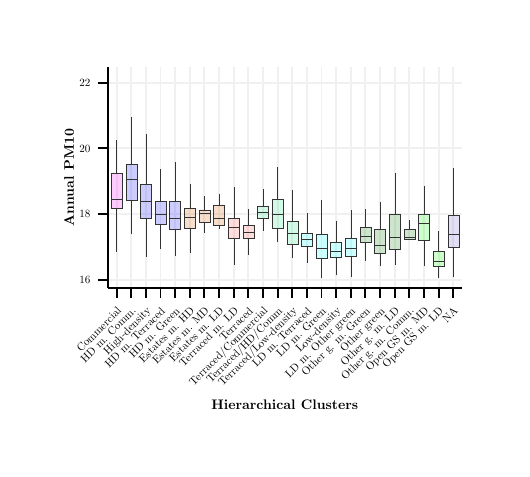
\begin{tikzpicture}[x=1pt,y=1pt]
\definecolor{fillColor}{RGB}{255,255,255}
\path[use as bounding box,fill=fillColor,fill opacity=0.00] (0,0) rectangle (171.17,152.15);
\begin{scope}
\path[clip] (  0.00,  0.00) rectangle (171.17,152.15);
\definecolor{fillColor}{RGB}{255,255,255}

\path[fill=fillColor] (  0.00,  0.00) rectangle (171.17,152.15);
\end{scope}
\begin{scope}
\path[clip] ( 28.95, 58.04) rectangle (156.94,137.92);
\definecolor{fillColor}{RGB}{255,255,255}

\path[fill=fillColor] ( 28.95, 58.04) rectangle (156.94,137.92);
\definecolor{drawColor}{gray}{0.94}

\path[draw=drawColor,line width= 0.7pt,line join=round] ( 28.95, 61.05) --
	(156.94, 61.05);

\path[draw=drawColor,line width= 0.7pt,line join=round] ( 28.95, 84.80) --
	(156.94, 84.80);

\path[draw=drawColor,line width= 0.7pt,line join=round] ( 28.95,108.55) --
	(156.94,108.55);

\path[draw=drawColor,line width= 0.7pt,line join=round] ( 28.95,132.30) --
	(156.94,132.30);

\path[draw=drawColor,line width= 0.7pt,line join=round] ( 32.12, 58.04) --
	( 32.12,137.92);

\path[draw=drawColor,line width= 0.7pt,line join=round] ( 37.41, 58.04) --
	( 37.41,137.92);

\path[draw=drawColor,line width= 0.7pt,line join=round] ( 42.70, 58.04) --
	( 42.70,137.92);

\path[draw=drawColor,line width= 0.7pt,line join=round] ( 47.99, 58.04) --
	( 47.99,137.92);

\path[draw=drawColor,line width= 0.7pt,line join=round] ( 53.28, 58.04) --
	( 53.28,137.92);

\path[draw=drawColor,line width= 0.7pt,line join=round] ( 58.57, 58.04) --
	( 58.57,137.92);

\path[draw=drawColor,line width= 0.7pt,line join=round] ( 63.85, 58.04) --
	( 63.85,137.92);

\path[draw=drawColor,line width= 0.7pt,line join=round] ( 69.14, 58.04) --
	( 69.14,137.92);

\path[draw=drawColor,line width= 0.7pt,line join=round] ( 74.43, 58.04) --
	( 74.43,137.92);

\path[draw=drawColor,line width= 0.7pt,line join=round] ( 79.72, 58.04) --
	( 79.72,137.92);

\path[draw=drawColor,line width= 0.7pt,line join=round] ( 85.01, 58.04) --
	( 85.01,137.92);

\path[draw=drawColor,line width= 0.7pt,line join=round] ( 90.30, 58.04) --
	( 90.30,137.92);

\path[draw=drawColor,line width= 0.7pt,line join=round] ( 95.59, 58.04) --
	( 95.59,137.92);

\path[draw=drawColor,line width= 0.7pt,line join=round] (100.88, 58.04) --
	(100.88,137.92);

\path[draw=drawColor,line width= 0.7pt,line join=round] (106.17, 58.04) --
	(106.17,137.92);

\path[draw=drawColor,line width= 0.7pt,line join=round] (111.45, 58.04) --
	(111.45,137.92);

\path[draw=drawColor,line width= 0.7pt,line join=round] (116.74, 58.04) --
	(116.74,137.92);

\path[draw=drawColor,line width= 0.7pt,line join=round] (122.03, 58.04) --
	(122.03,137.92);

\path[draw=drawColor,line width= 0.7pt,line join=round] (127.32, 58.04) --
	(127.32,137.92);

\path[draw=drawColor,line width= 0.7pt,line join=round] (132.61, 58.04) --
	(132.61,137.92);

\path[draw=drawColor,line width= 0.7pt,line join=round] (137.90, 58.04) --
	(137.90,137.92);

\path[draw=drawColor,line width= 0.7pt,line join=round] (143.19, 58.04) --
	(143.19,137.92);

\path[draw=drawColor,line width= 0.7pt,line join=round] (148.48, 58.04) --
	(148.48,137.92);

\path[draw=drawColor,line width= 0.7pt,line join=round] (153.77, 58.04) --
	(153.77,137.92);
\definecolor{drawColor}{gray}{0.20}

\path[draw=drawColor,line width= 0.1pt,line join=round] ( 37.41,102.83) -- ( 37.41,119.80);

\path[draw=drawColor,line width= 0.1pt,line join=round] ( 37.41, 89.93) -- ( 37.41, 77.73);
\definecolor{fillColor}{RGB}{0,0,255}

\path[draw=drawColor,line width= 0.1pt,fill=fillColor,fill opacity=0.20] ( 35.43,102.83) --
	( 35.43, 89.93) --
	( 39.39, 89.93) --
	( 39.39,102.83) --
	( 35.43,102.83) --
	cycle;

\path[draw=drawColor,line width= 0.1pt] ( 35.43, 97.31) -- ( 39.39, 97.31);

\path[draw=drawColor,line width= 0.1pt,line join=round] ( 42.70, 95.47) -- ( 42.70,113.70);

\path[draw=drawColor,line width= 0.1pt,line join=round] ( 42.70, 83.19) -- ( 42.70, 69.20);

\path[draw=drawColor,line width= 0.1pt,fill=fillColor,fill opacity=0.20] ( 40.72, 95.47) --
	( 40.72, 83.19) --
	( 44.68, 83.19) --
	( 44.68, 95.47) --
	( 40.72, 95.47) --
	cycle;

\path[draw=drawColor,line width= 0.1pt] ( 40.72, 89.43) -- ( 44.68, 89.43);

\path[draw=drawColor,line width= 0.1pt,line join=round] ( 32.12, 99.56) -- ( 32.12,111.42);

\path[draw=drawColor,line width= 0.1pt,line join=round] ( 32.12, 86.87) -- ( 32.12, 71.25);
\definecolor{fillColor}{RGB}{255,0,255}

\path[draw=drawColor,line width= 0.1pt,fill=fillColor,fill opacity=0.20] ( 30.14, 99.56) --
	( 30.14, 86.87) --
	( 34.10, 86.87) --
	( 34.10, 99.56) --
	( 30.14, 99.56) --
	cycle;

\path[draw=drawColor,line width= 0.1pt] ( 30.14, 90.35) -- ( 34.10, 90.35);

\path[draw=drawColor,line width= 0.1pt,line join=round] (100.88, 77.95) -- (100.88, 85.09);

\path[draw=drawColor,line width= 0.1pt,line join=round] (100.88, 73.08) -- (100.88, 67.22);
\definecolor{fillColor}{RGB}{0,255,255}

\path[draw=drawColor,line width= 0.1pt,fill=fillColor,fill opacity=0.20] ( 98.89, 77.95) --
	( 98.89, 73.08) --
	(102.86, 73.08) --
	(102.86, 77.95) --
	( 98.89, 77.95) --
	cycle;

\path[draw=drawColor,line width= 0.1pt] ( 98.89, 75.56) -- (102.86, 75.56);

\path[draw=drawColor,line width= 0.1pt,line join=round] (106.17, 77.39) -- (106.17, 89.91);

\path[draw=drawColor,line width= 0.1pt,line join=round] (106.17, 68.94) -- (106.17, 61.67);

\path[draw=drawColor,line width= 0.1pt,fill=fillColor,fill opacity=0.20] (104.18, 77.39) --
	(104.18, 68.94) --
	(108.15, 68.94) --
	(108.15, 77.39) --
	(104.18, 77.39) --
	cycle;

\path[draw=drawColor,line width= 0.1pt] (104.18, 72.52) -- (108.15, 72.52);

\path[draw=drawColor,line width= 0.1pt,line join=round] (132.61, 84.77) -- (132.61, 99.68);

\path[draw=drawColor,line width= 0.1pt,line join=round] (132.61, 72.29) -- (132.61, 66.45);
\definecolor{fillColor}{RGB}{0,128,0}

\path[draw=drawColor,line width= 0.1pt,fill=fillColor,fill opacity=0.20] (130.63, 84.77) --
	(130.63, 72.29) --
	(134.59, 72.29) --
	(134.59, 84.77) --
	(130.63, 84.77) --
	cycle;

\path[draw=drawColor,line width= 0.1pt] (130.63, 76.39) -- (134.59, 76.39);

\path[draw=drawColor,line width= 0.1pt,line join=round] ( 74.43, 83.48) -- ( 74.43, 94.43);

\path[draw=drawColor,line width= 0.1pt,line join=round] ( 74.43, 76.14) -- ( 74.43, 66.22);
\definecolor{fillColor}{RGB}{255,85,85}

\path[draw=drawColor,line width= 0.1pt,fill=fillColor,fill opacity=0.20] ( 72.45, 83.48) --
	( 72.45, 76.14) --
	( 76.42, 76.14) --
	( 76.42, 83.48) --
	( 72.45, 83.48) --
	cycle;

\path[draw=drawColor,line width= 0.1pt] ( 72.45, 79.97) -- ( 76.42, 79.97);

\path[draw=drawColor,line width= 0.1pt,line join=round] ( 53.28, 89.39) -- ( 53.28,103.47);

\path[draw=drawColor,line width= 0.1pt,line join=round] ( 53.28, 79.46) -- ( 53.28, 69.69);
\definecolor{fillColor}{RGB}{0,0,255}

\path[draw=drawColor,line width= 0.1pt,fill=fillColor,fill opacity=0.20] ( 51.29, 89.39) --
	( 51.29, 79.46) --
	( 55.26, 79.46) --
	( 55.26, 89.39) --
	( 51.29, 89.39) --
	cycle;

\path[draw=drawColor,line width= 0.1pt] ( 51.29, 83.39) -- ( 55.26, 83.39);

\path[draw=drawColor,line width= 0.1pt,line join=round] ( 79.72, 80.94) -- ( 79.72, 86.76);

\path[draw=drawColor,line width= 0.1pt,line join=round] ( 79.72, 76.12) -- ( 79.72, 70.12);
\definecolor{fillColor}{RGB}{255,85,85}

\path[draw=drawColor,line width= 0.1pt,fill=fillColor,fill opacity=0.20] ( 77.74, 80.94) --
	( 77.74, 76.12) --
	( 81.70, 76.12) --
	( 81.70, 80.94) --
	( 77.74, 80.94) --
	cycle;

\path[draw=drawColor,line width= 0.1pt] ( 77.74, 78.41) -- ( 81.70, 78.41);

\path[draw=drawColor,line width= 0.1pt,line join=round] ( 47.99, 89.40) -- ( 47.99,101.10);

\path[draw=drawColor,line width= 0.1pt,line join=round] ( 47.99, 81.19) -- ( 47.99, 72.03);
\definecolor{fillColor}{RGB}{0,0,255}

\path[draw=drawColor,line width= 0.1pt,fill=fillColor,fill opacity=0.20] ( 46.00, 89.40) --
	( 46.00, 81.19) --
	( 49.97, 81.19) --
	( 49.97, 89.40) --
	( 46.00, 89.40) --
	cycle;

\path[draw=drawColor,line width= 0.1pt] ( 46.00, 84.59) -- ( 49.97, 84.59);

\path[draw=drawColor,line width= 0.1pt,line join=round] (116.74, 76.25) -- (116.74, 86.27);

\path[draw=drawColor,line width= 0.1pt,line join=round] (116.74, 69.55) -- (116.74, 62.20);
\definecolor{fillColor}{RGB}{0,255,255}

\path[draw=drawColor,line width= 0.1pt,fill=fillColor,fill opacity=0.20] (114.76, 76.25) --
	(114.76, 69.55) --
	(118.73, 69.55) --
	(118.73, 76.25) --
	(114.76, 76.25) --
	cycle;

\path[draw=drawColor,line width= 0.1pt] (114.76, 72.57) -- (118.73, 72.57);

\path[draw=drawColor,line width= 0.1pt,line join=round] (111.45, 74.51) -- (111.45, 82.22);

\path[draw=drawColor,line width= 0.1pt,line join=round] (111.45, 69.35) -- (111.45, 62.77);

\path[draw=drawColor,line width= 0.1pt,fill=fillColor,fill opacity=0.20] (109.47, 74.51) --
	(109.47, 69.35) --
	(113.44, 69.35) --
	(113.44, 74.51) --
	(109.47, 74.51) --
	cycle;

\path[draw=drawColor,line width= 0.1pt] (109.47, 71.52) -- (113.44, 71.52);

\path[draw=drawColor,line width= 0.1pt,line join=round] (127.32, 79.24) -- (127.32, 89.19);

\path[draw=drawColor,line width= 0.1pt,line join=round] (127.32, 70.57) -- (127.32, 66.17);
\definecolor{fillColor}{RGB}{0,128,0}

\path[draw=drawColor,line width= 0.1pt,fill=fillColor,fill opacity=0.20] (125.34, 79.24) --
	(125.34, 70.57) --
	(129.30, 70.57) --
	(129.30, 79.24) --
	(125.34, 79.24) --
	cycle;

\path[draw=drawColor,line width= 0.1pt] (125.34, 73.45) -- (129.30, 73.45);

\path[draw=drawColor,line width= 0.1pt,line join=round] (122.03, 80.02) -- (122.03, 86.61);

\path[draw=drawColor,line width= 0.1pt,line join=round] (122.03, 74.49) -- (122.03, 67.79);

\path[draw=drawColor,line width= 0.1pt,fill=fillColor,fill opacity=0.20] (120.05, 80.02) --
	(120.05, 74.49) --
	(124.02, 74.49) --
	(124.02, 80.02) --
	(120.05, 80.02) --
	cycle;

\path[draw=drawColor,line width= 0.1pt] (120.05, 76.83) -- (124.02, 76.83);

\path[draw=drawColor,line width= 0.1pt,line join=round] ( 95.59, 82.30) -- ( 95.59, 93.36);

\path[draw=drawColor,line width= 0.1pt,line join=round] ( 95.59, 73.88) -- ( 95.59, 68.97);
\definecolor{fillColor}{RGB}{37,229,137}

\path[draw=drawColor,line width= 0.1pt,fill=fillColor,fill opacity=0.20] ( 93.60, 82.30) --
	( 93.60, 73.88) --
	( 97.57, 73.88) --
	( 97.57, 82.30) --
	( 93.60, 82.30) --
	cycle;

\path[draw=drawColor,line width= 0.1pt] ( 93.60, 77.86) -- ( 97.57, 77.86);

\path[draw=drawColor,line width= 0.1pt,line join=round] (148.48, 71.40) -- (148.48, 78.85);

\path[draw=drawColor,line width= 0.1pt,line join=round] (148.48, 65.80) -- (148.48, 61.83);
\definecolor{fillColor}{RGB}{0,255,0}

\path[draw=drawColor,line width= 0.1pt,fill=fillColor,fill opacity=0.20] (146.49, 71.40) --
	(146.49, 65.80) --
	(150.46, 65.80) --
	(150.46, 71.40) --
	(146.49, 71.40) --
	cycle;

\path[draw=drawColor,line width= 0.1pt] (146.49, 67.77) -- (150.46, 67.77);

\path[draw=drawColor,line width= 0.1pt,line join=round] ( 90.30, 90.09) -- ( 90.30,101.90);

\path[draw=drawColor,line width= 0.1pt,line join=round] ( 90.30, 79.63) -- ( 90.30, 74.58);
\definecolor{fillColor}{RGB}{37,229,137}

\path[draw=drawColor,line width= 0.1pt,fill=fillColor,fill opacity=0.20] ( 88.32, 90.09) --
	( 88.32, 79.63) --
	( 92.28, 79.63) --
	( 92.28, 90.09) --
	( 88.32, 90.09) --
	cycle;

\path[draw=drawColor,line width= 0.1pt] ( 88.32, 84.77) -- ( 92.28, 84.77);

\path[draw=drawColor,line width= 0.1pt,line join=round] ( 58.57, 87.01) -- ( 58.57, 95.62);

\path[draw=drawColor,line width= 0.1pt,line join=round] ( 58.57, 79.86) -- ( 58.57, 70.60);
\definecolor{fillColor}{RGB}{212,85,0}

\path[draw=drawColor,line width= 0.1pt,fill=fillColor,fill opacity=0.20] ( 56.58, 87.01) --
	( 56.58, 79.86) --
	( 60.55, 79.86) --
	( 60.55, 87.01) --
	( 56.58, 87.01) --
	cycle;

\path[draw=drawColor,line width= 0.1pt] ( 56.58, 83.53) -- ( 60.55, 83.53);

\path[draw=drawColor,line width= 0.1pt,line join=round] (143.19, 84.85) -- (143.19, 94.93);

\path[draw=drawColor,line width= 0.1pt,line join=round] (143.19, 75.22) -- (143.19, 65.96);
\definecolor{fillColor}{RGB}{0,255,0}

\path[draw=drawColor,line width= 0.1pt,fill=fillColor,fill opacity=0.20] (141.20, 84.85) --
	(141.20, 75.22) --
	(145.17, 75.22) --
	(145.17, 84.85) --
	(141.20, 84.85) --
	cycle;

\path[draw=drawColor,line width= 0.1pt] (141.20, 81.49) -- (145.17, 81.49);

\path[draw=drawColor,line width= 0.1pt,line join=round] ( 85.01, 87.68) -- ( 85.01, 93.83);

\path[draw=drawColor,line width= 0.1pt,line join=round] ( 85.01, 83.25) -- ( 85.01, 78.71);
\definecolor{fillColor}{RGB}{37,229,137}

\path[draw=drawColor,line width= 0.1pt,fill=fillColor,fill opacity=0.20] ( 83.03, 87.68) --
	( 83.03, 83.25) --
	( 86.99, 83.25) --
	( 86.99, 87.68) --
	( 83.03, 87.68) --
	cycle;

\path[draw=drawColor,line width= 0.1pt] ( 83.03, 85.34) -- ( 86.99, 85.34);

\path[draw=drawColor,line width= 0.1pt,line join=round] ( 63.85, 86.39) -- ( 63.85, 91.20);

\path[draw=drawColor,line width= 0.1pt,line join=round] ( 63.85, 82.02) -- ( 63.85, 78.00);
\definecolor{fillColor}{RGB}{212,85,0}

\path[draw=drawColor,line width= 0.1pt,fill=fillColor,fill opacity=0.20] ( 61.87, 86.39) --
	( 61.87, 82.02) --
	( 65.84, 82.02) --
	( 65.84, 86.39) --
	( 61.87, 86.39) --
	cycle;

\path[draw=drawColor,line width= 0.1pt] ( 61.87, 85.16) -- ( 65.84, 85.16);

\path[draw=drawColor,line width= 0.1pt,line join=round] ( 69.14, 87.89) -- ( 69.14, 91.87);

\path[draw=drawColor,line width= 0.1pt,line join=round] ( 69.14, 80.84) -- ( 69.14, 79.50);

\path[draw=drawColor,line width= 0.1pt,fill=fillColor,fill opacity=0.20] ( 67.16, 87.89) --
	( 67.16, 80.84) --
	( 71.13, 80.84) --
	( 71.13, 87.89) --
	( 67.16, 87.89) --
	cycle;

\path[draw=drawColor,line width= 0.1pt] ( 67.16, 83.38) -- ( 71.13, 83.38);

\path[draw=drawColor,line width= 0.1pt,line join=round] (137.90, 79.51) -- (137.90, 82.69);

\path[draw=drawColor,line width= 0.1pt,line join=round] (137.90, 75.79) -- (137.90, 75.25);
\definecolor{fillColor}{RGB}{0,128,0}

\path[draw=drawColor,line width= 0.1pt,fill=fillColor,fill opacity=0.20] (135.92, 79.51) --
	(135.92, 75.79) --
	(139.88, 75.79) --
	(139.88, 79.51) --
	(135.92, 79.51) --
	cycle;

\path[draw=drawColor,line width= 0.1pt] (135.92, 76.33) -- (139.88, 76.33);

\path[draw=drawColor,line width= 0.1pt,line join=round] (153.77, 84.50) -- (153.77,101.53);

\path[draw=drawColor,line width= 0.1pt,line join=round] (153.77, 72.91) -- (153.77, 61.95);
\definecolor{fillColor}{RGB}{106,90,205}

\path[draw=drawColor,line width= 0.1pt,fill=fillColor,fill opacity=0.20] (151.78, 84.50) --
	(151.78, 72.91) --
	(155.75, 72.91) --
	(155.75, 84.50) --
	(151.78, 84.50) --
	cycle;

\path[draw=drawColor,line width= 0.1pt] (151.78, 77.71) -- (155.75, 77.71);

\path[] ( 28.95, 58.04) rectangle (156.94,137.92);
\end{scope}
\begin{scope}
\path[clip] (  0.00,  0.00) rectangle (171.17,152.15);
\definecolor{drawColor}{RGB}{0,0,0}

\path[draw=drawColor,line width= 0.7pt,line join=round] ( 28.95, 58.04) --
	( 28.95,137.92);
\end{scope}
\begin{scope}
\path[clip] (  0.00,  0.00) rectangle (171.17,152.15);
\definecolor{drawColor}{RGB}{0,0,0}

\node[text=drawColor,anchor=base east,inner sep=0pt, outer sep=0pt, scale=  0.40] at ( 22.65, 59.67) {16};

\node[text=drawColor,anchor=base east,inner sep=0pt, outer sep=0pt, scale=  0.40] at ( 22.65, 83.42) {18};

\node[text=drawColor,anchor=base east,inner sep=0pt, outer sep=0pt, scale=  0.40] at ( 22.65,107.17) {20};

\node[text=drawColor,anchor=base east,inner sep=0pt, outer sep=0pt, scale=  0.40] at ( 22.65,130.92) {22};
\end{scope}
\begin{scope}
\path[clip] (  0.00,  0.00) rectangle (171.17,152.15);
\definecolor{drawColor}{RGB}{0,0,0}

\path[draw=drawColor,line width= 0.7pt,line join=round] ( 25.45, 61.05) --
	( 28.95, 61.05);

\path[draw=drawColor,line width= 0.7pt,line join=round] ( 25.45, 84.80) --
	( 28.95, 84.80);

\path[draw=drawColor,line width= 0.7pt,line join=round] ( 25.45,108.55) --
	( 28.95,108.55);

\path[draw=drawColor,line width= 0.7pt,line join=round] ( 25.45,132.30) --
	( 28.95,132.30);
\end{scope}
\begin{scope}
\path[clip] (  0.00,  0.00) rectangle (171.17,152.15);
\definecolor{drawColor}{RGB}{0,0,0}

\path[draw=drawColor,line width= 0.7pt,line join=round] ( 28.95, 58.04) --
	(156.94, 58.04);
\end{scope}
\begin{scope}
\path[clip] (  0.00,  0.00) rectangle (171.17,152.15);
\definecolor{drawColor}{RGB}{0,0,0}

\path[draw=drawColor,line width= 0.7pt,line join=round] ( 32.12, 54.54) --
	( 32.12, 58.04);

\path[draw=drawColor,line width= 0.7pt,line join=round] ( 37.41, 54.54) --
	( 37.41, 58.04);

\path[draw=drawColor,line width= 0.7pt,line join=round] ( 42.70, 54.54) --
	( 42.70, 58.04);

\path[draw=drawColor,line width= 0.7pt,line join=round] ( 47.99, 54.54) --
	( 47.99, 58.04);

\path[draw=drawColor,line width= 0.7pt,line join=round] ( 53.28, 54.54) --
	( 53.28, 58.04);

\path[draw=drawColor,line width= 0.7pt,line join=round] ( 58.57, 54.54) --
	( 58.57, 58.04);

\path[draw=drawColor,line width= 0.7pt,line join=round] ( 63.85, 54.54) --
	( 63.85, 58.04);

\path[draw=drawColor,line width= 0.7pt,line join=round] ( 69.14, 54.54) --
	( 69.14, 58.04);

\path[draw=drawColor,line width= 0.7pt,line join=round] ( 74.43, 54.54) --
	( 74.43, 58.04);

\path[draw=drawColor,line width= 0.7pt,line join=round] ( 79.72, 54.54) --
	( 79.72, 58.04);

\path[draw=drawColor,line width= 0.7pt,line join=round] ( 85.01, 54.54) --
	( 85.01, 58.04);

\path[draw=drawColor,line width= 0.7pt,line join=round] ( 90.30, 54.54) --
	( 90.30, 58.04);

\path[draw=drawColor,line width= 0.7pt,line join=round] ( 95.59, 54.54) --
	( 95.59, 58.04);

\path[draw=drawColor,line width= 0.7pt,line join=round] (100.88, 54.54) --
	(100.88, 58.04);

\path[draw=drawColor,line width= 0.7pt,line join=round] (106.17, 54.54) --
	(106.17, 58.04);

\path[draw=drawColor,line width= 0.7pt,line join=round] (111.45, 54.54) --
	(111.45, 58.04);

\path[draw=drawColor,line width= 0.7pt,line join=round] (116.74, 54.54) --
	(116.74, 58.04);

\path[draw=drawColor,line width= 0.7pt,line join=round] (122.03, 54.54) --
	(122.03, 58.04);

\path[draw=drawColor,line width= 0.7pt,line join=round] (127.32, 54.54) --
	(127.32, 58.04);

\path[draw=drawColor,line width= 0.7pt,line join=round] (132.61, 54.54) --
	(132.61, 58.04);

\path[draw=drawColor,line width= 0.7pt,line join=round] (137.90, 54.54) --
	(137.90, 58.04);

\path[draw=drawColor,line width= 0.7pt,line join=round] (143.19, 54.54) --
	(143.19, 58.04);

\path[draw=drawColor,line width= 0.7pt,line join=round] (148.48, 54.54) --
	(148.48, 58.04);

\path[draw=drawColor,line width= 0.7pt,line join=round] (153.77, 54.54) --
	(153.77, 58.04);
\end{scope}
\begin{scope}
\path[clip] (  0.00,  0.00) rectangle (171.17,152.15);
\definecolor{drawColor}{RGB}{0,0,0}

\node[text=drawColor,rotate= 45.00,anchor=base east,inner sep=0pt, outer sep=0pt, scale=  0.40] at ( 34.05, 49.51) {Commercial};

\node[text=drawColor,rotate= 45.00,anchor=base east,inner sep=0pt, outer sep=0pt, scale=  0.40] at ( 39.34, 49.51) {HD m. Comm.};

\node[text=drawColor,rotate= 45.00,anchor=base east,inner sep=0pt, outer sep=0pt, scale=  0.40] at ( 44.63, 49.51) {High-density};

\node[text=drawColor,rotate= 45.00,anchor=base east,inner sep=0pt, outer sep=0pt, scale=  0.40] at ( 49.92, 49.51) {HD m. Terraced};

\node[text=drawColor,rotate= 45.00,anchor=base east,inner sep=0pt, outer sep=0pt, scale=  0.40] at ( 55.21, 49.51) {HD m. Green};

\node[text=drawColor,rotate= 45.00,anchor=base east,inner sep=0pt, outer sep=0pt, scale=  0.40] at ( 60.49, 49.51) {Estates m. HD};

\node[text=drawColor,rotate= 45.00,anchor=base east,inner sep=0pt, outer sep=0pt, scale=  0.40] at ( 65.78, 49.51) {Estates m. MD};

\node[text=drawColor,rotate= 45.00,anchor=base east,inner sep=0pt, outer sep=0pt, scale=  0.40] at ( 71.07, 49.51) {Estates m. LD};

\node[text=drawColor,rotate= 45.00,anchor=base east,inner sep=0pt, outer sep=0pt, scale=  0.40] at ( 76.36, 49.51) {Terraced m. LD};

\node[text=drawColor,rotate= 45.00,anchor=base east,inner sep=0pt, outer sep=0pt, scale=  0.40] at ( 81.65, 49.51) {Terraced};

\node[text=drawColor,rotate= 45.00,anchor=base east,inner sep=0pt, outer sep=0pt, scale=  0.40] at ( 86.94, 49.51) {Terraced/Commercial};

\node[text=drawColor,rotate= 45.00,anchor=base east,inner sep=0pt, outer sep=0pt, scale=  0.40] at ( 92.23, 49.51) {Terraced/HD/Comm};

\node[text=drawColor,rotate= 45.00,anchor=base east,inner sep=0pt, outer sep=0pt, scale=  0.40] at ( 97.52, 49.51) {Terraced/Low-density};

\node[text=drawColor,rotate= 45.00,anchor=base east,inner sep=0pt, outer sep=0pt, scale=  0.40] at (102.81, 49.51) {LD m. Terraced};

\node[text=drawColor,rotate= 45.00,anchor=base east,inner sep=0pt, outer sep=0pt, scale=  0.40] at (108.09, 49.51) {LD m. Green};

\node[text=drawColor,rotate= 45.00,anchor=base east,inner sep=0pt, outer sep=0pt, scale=  0.40] at (113.38, 49.51) {Low-density};

\node[text=drawColor,rotate= 45.00,anchor=base east,inner sep=0pt, outer sep=0pt, scale=  0.40] at (118.67, 49.51) {LD m. Other green};

\node[text=drawColor,rotate= 45.00,anchor=base east,inner sep=0pt, outer sep=0pt, scale=  0.40] at (123.96, 49.51) {Other g. m. Green};

\node[text=drawColor,rotate= 45.00,anchor=base east,inner sep=0pt, outer sep=0pt, scale=  0.40] at (129.25, 49.51) {Other green};

\node[text=drawColor,rotate= 45.00,anchor=base east,inner sep=0pt, outer sep=0pt, scale=  0.40] at (134.54, 49.51) {Other g. m. LD};

\node[text=drawColor,rotate= 45.00,anchor=base east,inner sep=0pt, outer sep=0pt, scale=  0.40] at (139.83, 49.51) {Other g. m. Comm.};

\node[text=drawColor,rotate= 45.00,anchor=base east,inner sep=0pt, outer sep=0pt, scale=  0.40] at (145.12, 49.51) {Open GS m. MD};

\node[text=drawColor,rotate= 45.00,anchor=base east,inner sep=0pt, outer sep=0pt, scale=  0.40] at (150.41, 49.51) {Open GS m. LD};

\node[text=drawColor,rotate= 45.00,anchor=base east,inner sep=0pt, outer sep=0pt, scale=  0.40] at (155.69, 49.51) {NA};
\end{scope}
\begin{scope}
\path[clip] (  0.00,  0.00) rectangle (171.17,152.15);
\definecolor{drawColor}{RGB}{0,0,0}

\node[text=drawColor,anchor=base,inner sep=0pt, outer sep=0pt, scale=  0.50] at ( 92.94, 14.03) {\bfseries Hierarchical Clusters};
\end{scope}
\begin{scope}
\path[clip] (  0.00,  0.00) rectangle (171.17,152.15);
\definecolor{drawColor}{RGB}{0,0,0}

\node[text=drawColor,rotate= 90.00,anchor=base,inner sep=0pt, outer sep=0pt, scale=  0.50] at ( 16.70, 97.98) {\bfseries Annual PM10};
\end{scope}
\end{tikzpicture}
